\documentclass{article}
\usepackage{hyperref}
\usepackage{color}
\usepackage{graphicx}
\addtolength{\oddsidemargin}{-.875in}
\addtolength{\evensidemargin}{-.875in}
\addtolength{\textwidth}{1.75in}
\addtolength{\topmargin}{-.875in}
\addtolength{\textheight}{1.75in}

\pagestyle{plain}
\author{Rahul Daware}
\begin{document}
\title{Chapter 8 : VPC Overview}
\maketitle
\newpage
\tableofcontents
\newpage

\section{What is VPC?}
Think of VPC as a virtual data center in the cloud. Amazon Virtual Private Cloud (Amazon VPC) lets you provision a logically isolated section of  the Amazon Web Service (AWS) cloud where you can launch AWS resources in a virtual network that you define. You have complete control over your virtual networking environment, including selection of your own IP address range, creation of subnets, and configuration of route tables and network gateways. Additionally, you can create a hardware Virtual Private Network (VPN) connection between your coroporate datacenter and your VPC and leverage the AWS cloud as an extension of your corporate datacenter.

\begin{figure}

  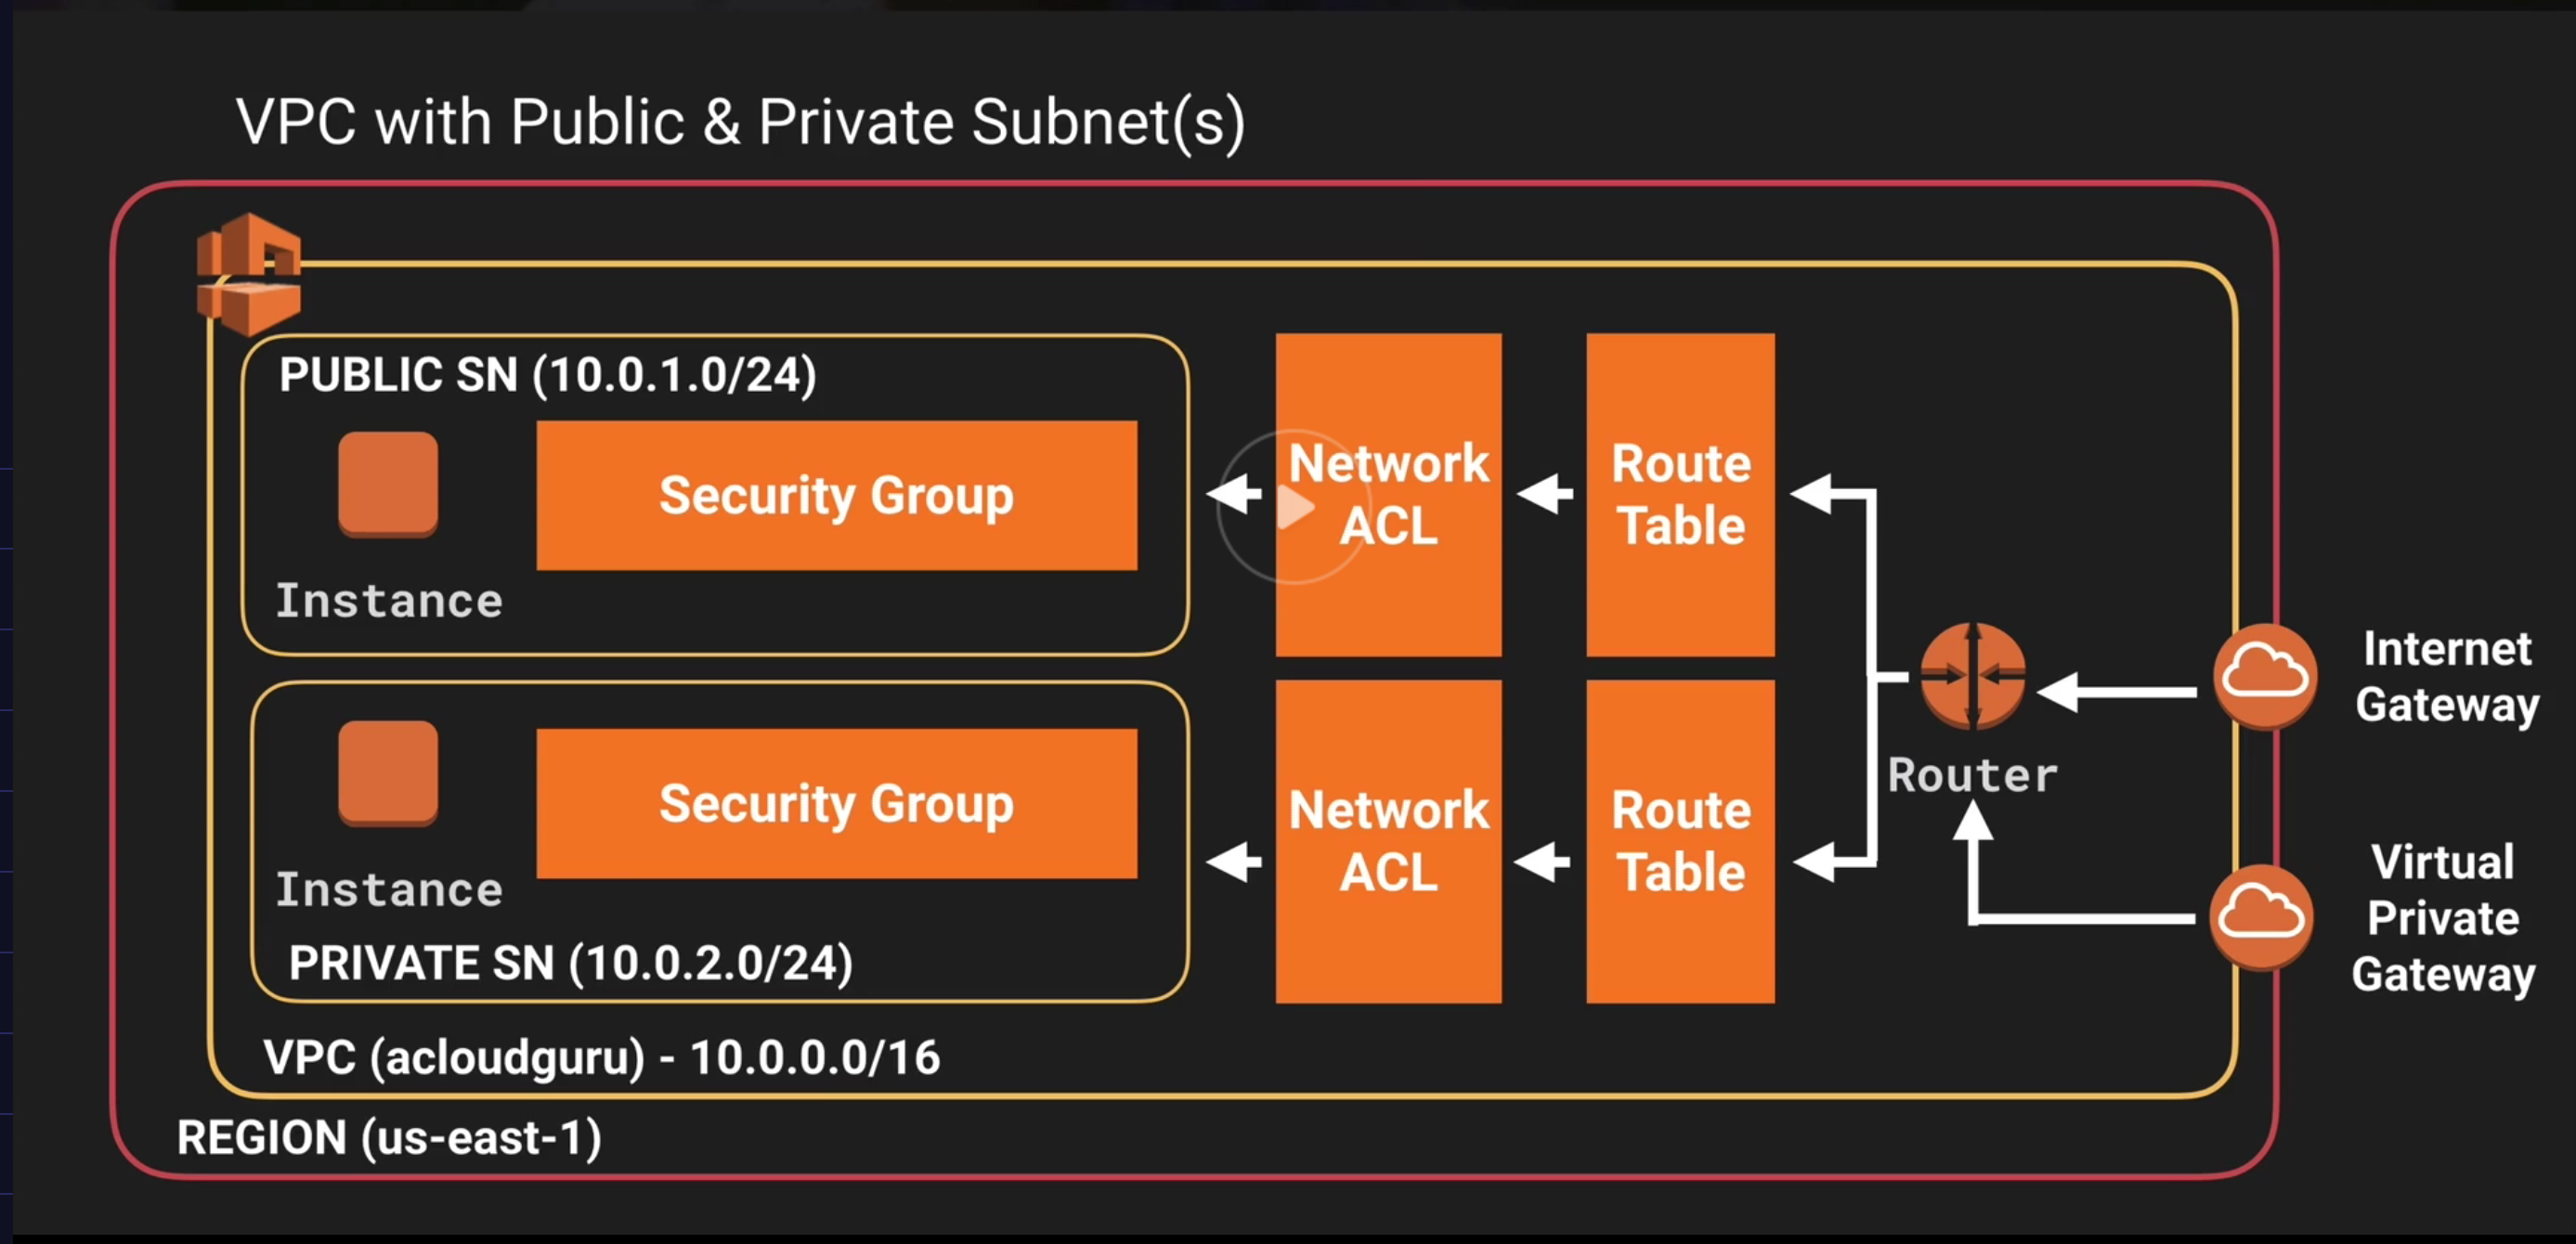
\includegraphics[width =\linewidth]{images/vpc1.png}
  \caption{VPC Diagram}
  \label{fig:VPC Diagram}
\end{figure}

\subsection{What can you do with a VPC?}
\begin{itemize}
\item
Launch instances into a subnet of your choosing

\item
Assign custom IP address ranges in each subnet

\item
Configure route tables between subnets

\item
Create internet gateway and attach it to our VPC

\item
Much better security control over your AWS resources

\item
Instance security groups

\item
Subnet network access control lists (ACLs)

\end{itemize}

\subsection{Default VPC}
\begin{itemize}
\item
Default VPC is user friendly, allowing you to immediately deploy instances

\item
All subnets in default VPC have a route out to the internet

\item
Each EC2 instance has both a public and private IP address

\end{itemize}

\subsection{VPC Peering}
\begin{itemize}
\item
Allows you to connect one VPC with another via a direct network route using private IP addresses

\item
Instances behave as if they were on the same private network

\item
You can peer VPCs with other AWS accounts as well as with other VPCs in the same account

\item
Peering is in a star configuration. i.e. 1 central VPC peers with 4 others. No transitive peering

\end{itemize}

\subsection{Exam Tips}

\begin{itemize}
\item
Think of a VPC as a logical datacenter in AWS

\item
Consists of IGWs (or Virtual Private Gateways), Route Tables , Network Access Control Lists, Subnets, and Security Groups

\item
1 subnet = 1 availability zone

\item
Security groups are stateful, network access control lists are stateless

\item
No transitive peering


\end{itemize}
\end{document}